\documentclass[../../main.tex]{subfiles}
\begin{document}

\subsection*{8.6}
Nei due circuiti in figura i raggi delle semicirconferenze sono $a=10\ cm$ e $b=15\ cm$.\\
a) Se la corrente vale $i = 20\ A$ calcolare per entrambi il campo magnetico $\vec{B_0}$ nel centro O delle semicirconferenze.\\
b) Calcolare il momento magnetico $\vec{m}$.\\
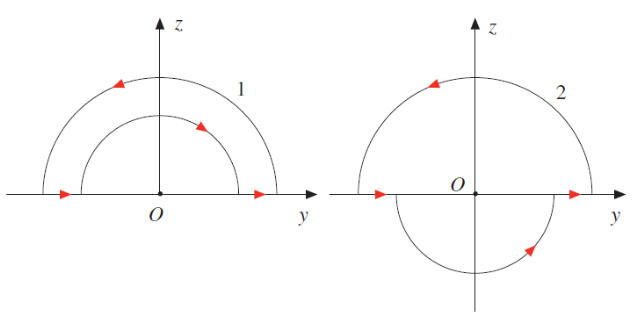
\includegraphics[scale=0.3]{e_8_6.png}
\subsubsection*{Formule utilizzate}
\subsubsection*{Soluzione punto a}
Il campo magnetico in O generato da ogni semicerchio si trova dimezzando l'espressione del camo di una spira circolare al centro della spira oppure applicando direttamente la prima legge elementare di Laplace.\\
Nominando i 4 punti sull'asse y come A, B, C, D partendo da sinistra:\\
$\vec{B_{AB}}(O) = \vec{B_{CD}}(O) = 0$ poichè paralleli a $\vec{u_r}$\\
$\vec{B_{BC}}(O) = \int_B^C\frac{\mu_0i}{4\pi}\frac{ds\wedge\vec{u_r}}{r^2}=\frac{\mu_0i}{4\pi a^2}\int_B^Cds (-\vec{u_x})$ con $\int_B^C = \pi a$\\
Stesso procedimento per $\vec{B_{DA}}$ ma con direzione $\vec{u_x}$\\
$\vec{B_0} = \frac{\mu_0 i}{4b}\vec{u_x}-\frac{\mu_0 i}{4a}\vec{u_x}$\\
essendo che i due tratti rettilinei danno contributo nullo $(d\vec{s} \parallel \vec{u_r})$.\\
Numericamente:\\
$B_O = \frac{1.26 * 10^{-6} * 20}{4}\left(\frac{1}{0.15}-\frac{1}{0.1}\right) = -2.1 * 10^{-5}\ T$\\\\
Per il secondo campo:\\
$\vec{B_{AB}}$, $\vec{B_{CD}}$, $\vec{B_{DA}}$ sono uguali a prima, mentre $\vec{B_{BC}}$ ha segno opposto.\\
$\vec{B_0} = \frac{\mu_0 i}{4b}\vec{u_x}+\frac{\mu_0 i}{4a}\vec{u_x}$\\
Numericamente:\\
$B_0 = \frac{1.26 * 10^{-6} * 20}{4}\left(\frac{1}{0.15}+\frac{1}{0.1}\right) = 10.5* 10^{-5}\ T$\\


\subsubsection*{Soluzione punto b}
Nella prima situazione:\\
$\vec{m} = i\frac{\pi}{2}\left(b^2 - a^2\right)\vec{u_x}=0.39\vec{u_x}\ Am^2$\\
Nella seconda situazione:\\
$\vec{m} = i\frac{\pi}{2}\left(b^2 + a^2\right)\vec{u_x}=1.02\vec{u_x}\ Am^2$
\newpage

\end{document}